% this file is called up by thesis.tex
% content in this file will be fed into the main document
\chapter{Knowledge Based Design} % top level followed by section, subsection
%: ----------------------- paths to graphics ------------------------

% change according to folder and file names
\ifpdf
    \graphicspath{{3/figures/PNG/}{3/figures/PDF/}{2.5/figures/}}
\else
    \graphicspath{{3/figures/EPS/}{3/figures/}}
\fi

%: ----------------------- contents from here ------------------------

A new design methodology, named Knowledge Based Design (KBD), that combines EAs with Knowledge-based systems (KBS)  is proposed in this thesis. This methodology uses a KBS system similar to Case-Based Reasoning (CBR) in order to utilise/exploit the availability, in any industrial environment, of a database of previous "good" design/s. In the design of fluid dynamic shapes a pattern of similar geometries often occurs when dealing with similar problems. That gives rise to the notion that even if a design is optimal for a set of different/neighbouring conditions it still holds valuable information about the design space that can be exploited in order to speed up the design procedure. That is the purpose of the proposed KBD method.  

From KBS point of view the proposed methodology achieves in creating a fully automated and time efficient revise step, the step that adapts the older similar designs in order to perform optimally in the desired, new, conditions. This is achieved by using an EA as a revise/optimization tool. In order to have a time efficient procedure, acceptable in an industrial environment, a number of EA speed-up techniques, mainly the use of metamodels (MAEA, section.\ref{MAEApar}), are in use.  

Regarding EAs this method achieves three important goals: 
\begin{description}
  \item[a)]The significant reduction of the problem dimension ($N$ number of design variables) thus improving both EA efficiency (faster convergence) and MAEA efficiency (better accommodation of ANNs as metamodels (see.\ref{MAEApar})). 
  \item[b)]The automatic definition of the effective variables range thus freeing the engineer from the burden of "guestimating" them and eliminating the possibility of , by mistake, not including the real optimum design in the design space.
    \item[c)]The introduction of importance, i.e. higher probability to host a candidate solution in the design space, thus allowing the exploration of bigger design spaces but with different levels of importance for the regions of it.
\end{description}
All the above allow the exploitation of relatively big design spaces, both in number of design variables and effective range, in an efficient way exploiting the information that is incorporated in the availability of older "good: design operating at neighbouring conditions.     

\section{Knowledge-based Systems (KBS)}  
Knowledge-based systems (KBS) are systems based on the methods and techniques of artificial intelligence. Their core components are the knowledge base and inference mechanisms. In this thesis a KBS that resembles Case-Based Reasoning (CBR) is combined with EAs, in an optimal way, giving rise to the proposed KBD method. CBR can be seen as a problem solving method that reuses past cases and experience to conceive a solution to a current problem, 
while other major artificial intelligence techniques rely on mapping generalized 
relationships between problem descriptions and conclusions. CBR has the advantage 
of utilizing previous experience based on concrete old-problem solutions. 
The central tasks of a CBR system to identify the problem in hand, find one or 
more similar past case(s), use this information to suggest a solution to the current 
problem and update the system by learning from this experience \cite{kolodner_1991,kolodner_1993,slade_1991,riesbeck_1989}.      

%***********************************************************************
\subsection{Case-Based Reasoning}
%***********************************************************************
\label{History} The origins of CBR lay in the work of 
Schank and Abelson in 1977 \cite{Schank_Abelson_1977}. They proposed that general 
human knowledge about situations is recorded as scripts that allows the extract 
of expectations and inferences. Scripts were proposed as structure for conceptual 
memory describing information about stereotypical events. However, experiments 
showed that they are not a complete theory of memory representation since people 
often confuse events with similar scripts. Such observations fell in line with 
concept formulation, problem solving and experimental learning theories within 
philosophy and psychology \cite{tulving_1977,smith_1978}. 

Schank continued to investigate the role of previews situations (i.e. cases) 
and situation patterns role in both problem solving and learning \cite{Schank_1982},  
simultaneously Gentner \cite{genter_1983} was developing a  
theoretical framework for analogy also relevant to CBR. Significant references to CBR can also be fount in 
Wittgensteins's observation \cite{wittgestein_1953} that natural concepts are in fact 
polymorphic and can not be classified by a single set of necessary and sufficient 
features but instead can be defined by a set of instances (i.e. cases) with family 
resemblances. The latter work has been cited as the philosophical basis for CBR by Aamondt and Plaza \cite{aamond_plaza_1994}.

Even though the roots of CBR can be claimed by many, it was Schank and his group that in the early eighties produced a cognitive model where the first CBR applications were based upon. Kolonder developed the first CBR system named CYRUS \cite{kolodner_1983a,kolodner_1983b} which was an implementation of Schank's dynamic memory model. Its case-memory model later served as the basis for several other CBR systems finding use in a lot of disciplines raging from law \cite{ashley_1988,rissland_skalak_1989} to civil engineering \cite{whatson_abdullah_1994,moore_1994}.

\label {CBR}  The classic definition of CBR was coined by Riesbeck and Schank \cite{riesbeck_1989}: "A case-based reasoner solves problems by using or adapting solutions to old problems". Which answers exactly the what a CBR system should do but not the how it dose it. The answer to the second question is commonly described by the so called CBR-cycle (Figure \ref{cbr}).  The CBR-cycle is based on four logical steps, as described by Aamodt and Plaza \cite{aamond_plaza_1994}, comprising the four REs: 

\begin{itemize}
  \item RETRIEVE the most similar case(s);
  \item REUSE the case(s) to attempt to solve the problem;
  \item REVISE the proposed solution if necessary, and
  \item RETAIN the new solution in the Case-Base.
\end{itemize}
which can be represented by a schematic cycle (see Figure \ref{cbr}).

%\figuremacroW{cbr}{Schematic cycle representing the CBR-cycle}{0.5}
\begin{figure}[h!]
\begin{minipage}[b]{1\linewidth}
 \centering
 \resizebox*{!}{10 cm}{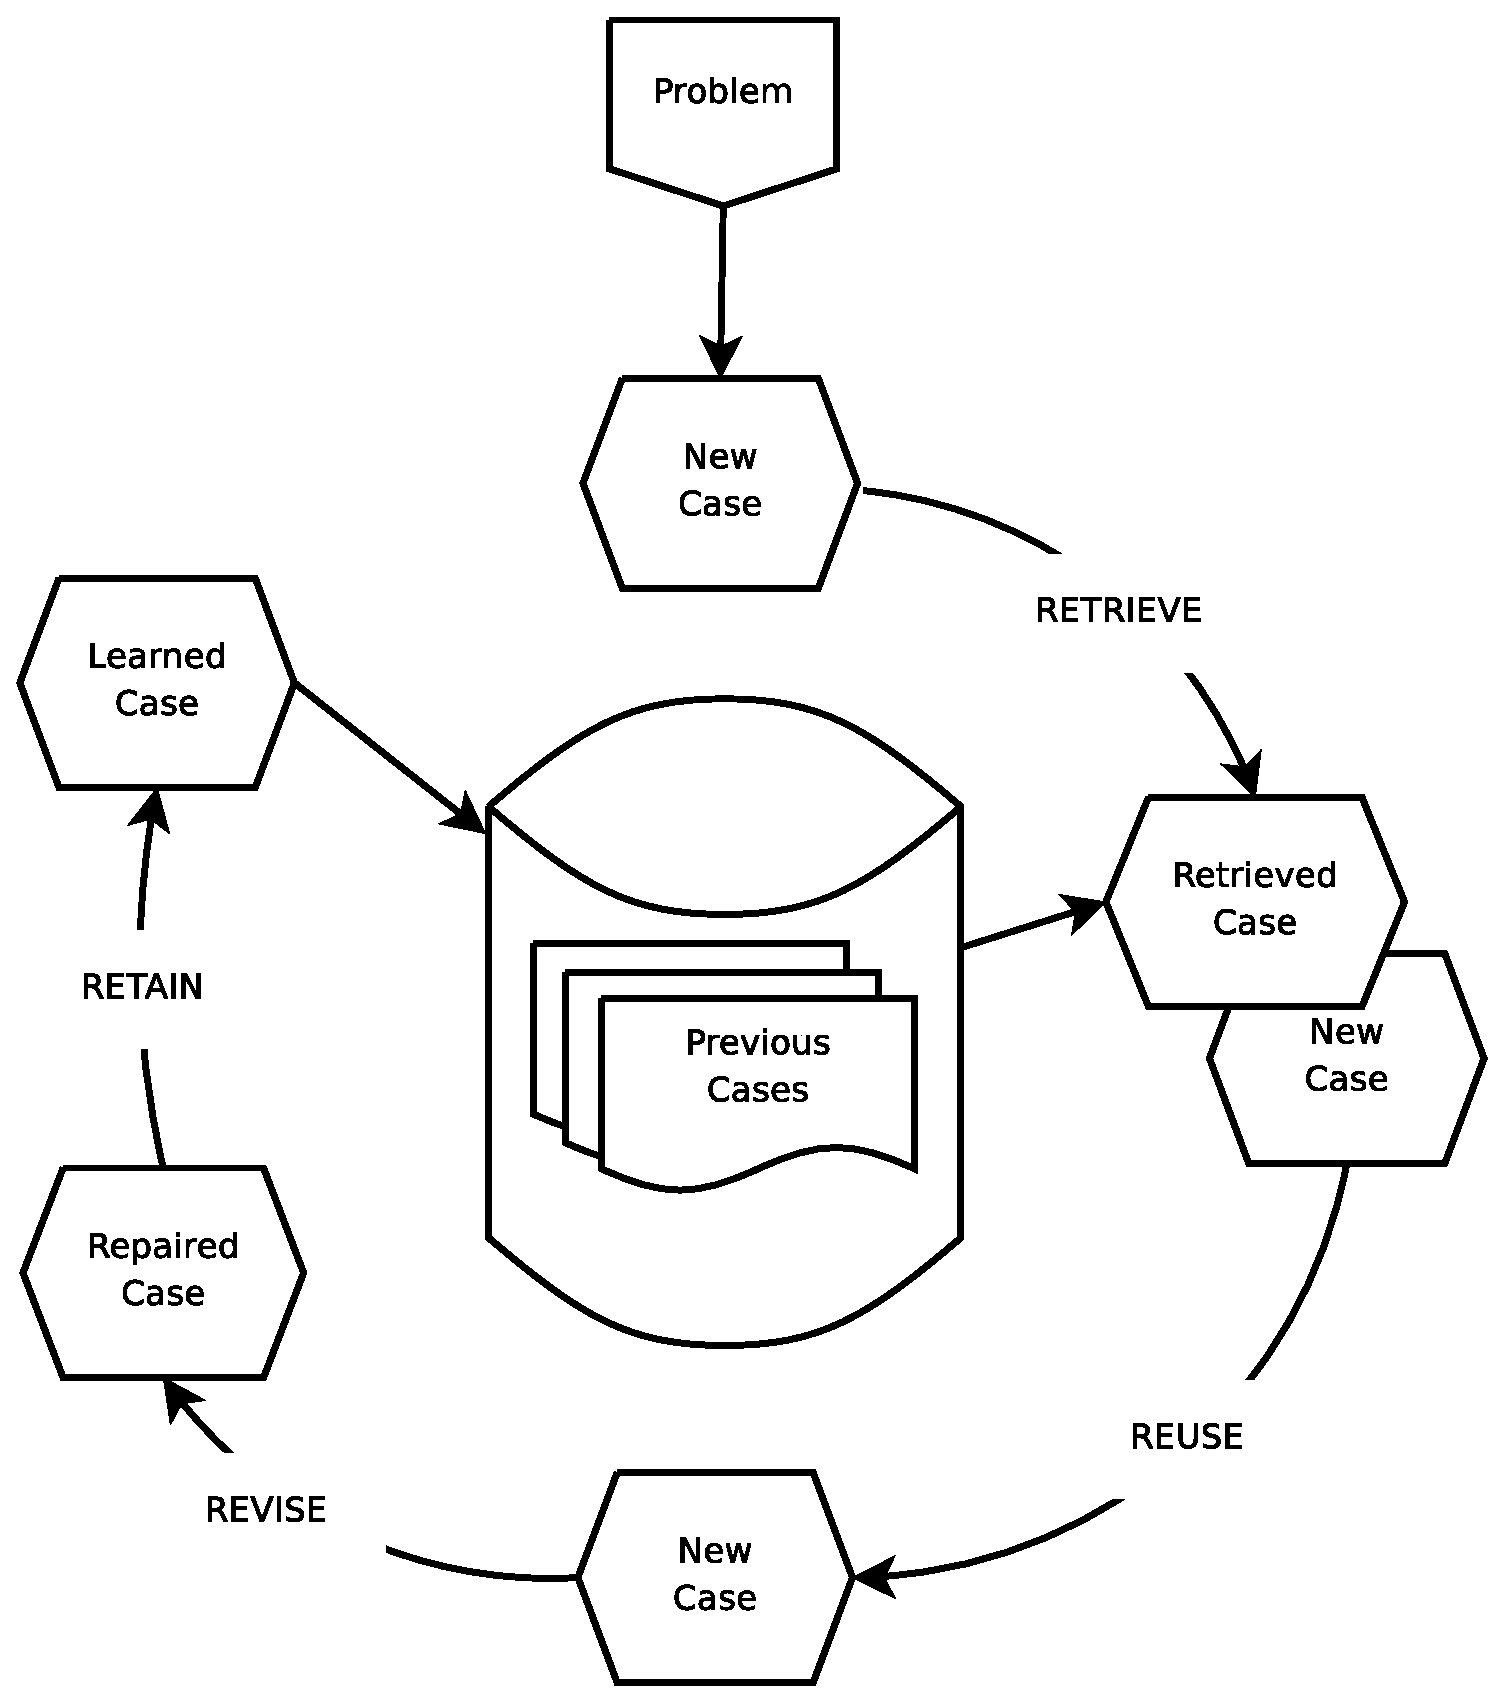
\includegraphics{cbr.eps}}
\end{minipage}
\caption{Schematic representation of the CBR-cycle.} 
\label{cbr}
\end{figure}

A new problem is matched against cases in the case database and thought a similarity 
criterion one or more similar cases are retrieved. A solution is suggested by the 
matching cases. This is then reused and tested for success. Unless the suggested solution 
is a close match it will probably have to be revised. In the end of this procedure the 
new case should be retained in the case-base. This cycle rarely is independent of 
human intervention. Many CBR tools act solely as case retrieval an reuse systems. 
Case revision (i.e. adaptation) is often left as a human task. Following the CBR-cycle processes are outlined.

%-----------------------------------------------------------------------
\subsubsection{Retrieve}
%-----------------------------------------------------------------------
\label{Retrieve} 
Given a description of a problem, a retrieval algorithm, using the indices in the case database (case-memory), 
should retrieve the most similar case(s) to the current problem or situation. The retrieval algorithm 
relies the organisation of the memory to direct the search to potentially useful cases.

The issue of choosing the best matching case has been addressed by research into analogy \cite{Falkenehainer_1986}. 
This approach involves using heuristics to constrain and direct the search. Several algorithms have 
been implemented to retrieve appropriate cases, such as: serial search 
\cite{Navinchandar_1991, Acorn_Walden_1992, Simoudis_93}, hierarchical search 
\cite{Maher_Zhang_1991} and simulated parallel search \cite{Domeshek_1993}.

Case-based reasoning can be used for large scale problems if combined with retrieval algorithms that are capable to handle thousands of cases. Unlike database searches that target a specific value in a record, retrieval of cases from the case database must be equipped with heuristics that perform partial matches, since in general there is no existing case that exactly matches the new case.

Among well known methods for case retrieval are: nearest neighbour, induction, 
knowledge guided induction and template retrieval. These methods can be used 
alone or combined into hybrid retrieval strategies.

\paragraph{Nearest neighbour}
\label{nearest neighbour}This approach involves the assessment of similarity 
between stored cases and the new input case, based on matching a weighted sum 
of features. The main problem here is to determine the weights of the features. 
The limitation of this approach include problems in converging on the 
correct solution and retrieval times. In general the use of this method leads 
to the retrieval time increasing linearly with the number of cases. Therefore 
this approach is more effective when the case base is relatively small. 

\paragraph{Induction}
\label{Induction}Induction algorithms determine which features do the best job 
in discriminating cases, and generate a decision tree-type structure to organise 
the cases in memory. This approach is useful when a single case feature is 
required as a solution, and where that case feature is dependent upon others.

\paragraph{Knowledge guided induction}
\label{Knowledge guided induction} This method applies knowledge to the induction 
process by manually identifying case features that are known or thought to affect 
the primary case feature. This approach is frequently used in conjunction with other 
techniques, because the explanatory knowledge is not always readily available for large case bases.

\paragraph{Template retrieval}
\label{template} Similar to SQL-like queries, template retrieval returns all 
cases that fit within certain parameters. This technique is often used before 
other techniques, such as nearest neighbour, to limit the search space to a 
relevant section of the case-base.

%-----------------------------------------------------------------------
\subsubsection{Revise - Adaptation}
%-----------------------------------------------------------------------
\label{Revise} Once a solution is suggested based on the matching retrieved case(s) 
a CBR system should adapt the solution to the needs of the current case. Adaptation 
looks for prominent differences between the proposed solution and the current case and 
then applies formulae or rules that take those differences into account when 
suggesting an improved solution. In general, an ideal set of adaptation rules must be strong enough to generate complete solutions from scratch.

\paragraph{}
Several techniques, ranging from simple to complex, have been used in CBR for adaptation. These include:

\paragraph{Null adaptation} A direct simple technique that applies whatever solution is retrieved to the current 
problem without adapting it. Null adaptation is useful for problems involving complex 
reasoning but with a simple solution. For example, when someone applies for a bank loan, 
after answering numerous questions the final answer is very simple: grant the loan, 
reject the loan, or refer the application.

\paragraph{Parameter adjustment} Compares specified parameters of the retrieved 
and current case to modify the solution in an appropriate direction.

\paragraph{Abstraction and respecialisation}
A general adaptation technique that is used in a basic way to achieve simple 
adaptations and in a complex way to generate novel, creative solutions.

\paragraph{Critic-based adaptation}
In which a critic looks for combinations of features that can cause a problem in 
a solution. Importantly, the critic is aware of repairs for these problems.

\paragraph{Reinstantiation}
Is used to instantiate features of an old solution with new features.

\paragraph{Derivational replay}
Is the process of using the method of deriving an old solution or solution piece to derive a solution in the new situation.

\paragraph{Model-guided repair}
Uses a causal model to guide adaptation.

\paragraph{Case-based substitution}
Uses cases to suggest solution adaptation.
%-----------------------------------------------------------------------
\subsubsection{Retain}
%-----------------------------------------------------------------------
\label{Retain} Case is a piece of knowledge representing an experience. This knowledge has to 
be retained in the case database after a successful procedure \cite{kolodner_1993}. Typically a case comprises:   
\begin{itemize}
	\item the problem that describes the state of the world when the case occurred.
	\item the solution which states the derived solution to that problem.
	\item the outcome which describe the state of the world after the case occurred. 
\end{itemize}

There is a lack of consensus within the CBR community on what information should be in a case. However its advised that two measures can be taken into account when deciding,
 the functionality and the ease of acquisition of the information represented in the case \cite{kolodner_1993}. 
%%%%%%%%%%%%%%%%%%%%%%%%%%%%%%%%%%%%%%%%%%%%%%%%%%%%%%%%%%%%%%%%%%%%%%%%

%%%%%%%%%%%%%%%%%%%%%%%%%%%%%%%%%%%%%%%%%%%%%%%%%%%%%%%%%%%%%%%%%%%%%%%

\section{The Knowledge Based Design method}

In case of design of fluid dynamic shaped with specific characteristics in a specific environment, due to the nature of the problem, the solution is always complex. Thus the need of adaptation (revise) is almost certain. \textit{Null adaptation is useful for problems involving complex reasoning but with a simple solution.}

In order to have a fully automated system, the role of human intervention in adaptation has to be replaced by a set of adaptation rules. These rules take into account the derivations of the proposed solution compared to the desired one and suggest an improved proposal. The rules that govern the evolution of species, ideally fit the above description. So an  evolutionary algorithm (EA) is a perfect tool to undertake the revise step. 

Therefore the method proposed in this thesis aims to extend the base optimization method by making it capable to accommodate and exploit pieces of useful information archived during previous relevant successful designs. So, instead of parameterizing the geometry, which inevitably leads to many design variables (especially in cases of complex three dimensional geometries like thermal and hydro turbines) thus slow down the design procedure, in the proposed method all new designs are expressed as weighted combinations of the archived ones. The archived designs act as the design space base. The role of the optimization algorithms is to find the set (or sets, for more than one objectives, where the Pareto front of non-dominated solutions is sought) of weight values, corresponding to the shape with optimal performance. Since the number of weights is much less that the number of design variables of the conventional shape parameterization, the design space dimension is reduced and the CPU cost of the EA/MAEA is much lower.

\subsection{Designing a new geometry based on archived designs}
Let us assume that a small number of previous designs are retrieved from the case database. These designs must have been performed for similar problems and archived with respect to all design variables, in conformity with the same parameterization. Let us denote by $GEO_i=(b_1^i,b_2^i,....,b_n^i)$, $i\!=\!1,m$ the m archived designs, with $b_j$, $j=1,n$  the “conventional” design variables. It is a simple matter to assume that any new design $b_j^{new}$ may result from the combination of $m$ archived designs, by means of weights $w_i (i=1,m)$. This is, in fact, equivalent to a multi-linear interpolation scheme, namely:

\begin{eqnarray}
   b_j^{new} = \frac{\sum_{i=1}^{m}w_i \times b_j^i}{\sum_{i=1}^{m}w_i } 
   \label{linear} 
\end{eqnarray}

Without loss in generality, we may assume that $w_i \in [0,1]$. Setting up an optimization method merely based on eq.\ref{linear} leads to a parsimonious set of unknowns (or design variables, namely the m values of $w_i$; recall that m is quite small compared to n). However, since (a) m is small and (b) a multi-linear interpolation with the same weight for all variables comprising the same archived design is used, the flexibility and effectiveness of such a method may become degraded. 

Among other, the set of the archived solutions reveals the statistical distribution of each design variable and, consequently, this can also be used to set the bounds of the design space. In place of eq. \ref{linear}, the nonlinear equations

\begin{eqnarray}
   b_j^{new} = \Phi _j^{-1} (\frac{\sum_{i=1}^{m}w_i \times \Phi _j(b_j^i)}{\sum_{i=1}^{m}w_i }) 
   \label{non-linear} 
\end{eqnarray}

can be used to define each new design. In eq. \ref{non-linear},$\Phi _j$ are appropriate nonlinear functions. Based on the assumption that the retrieved designs (which will also be referred to as design bases) correspond to operating conditions correlated to the new ones, the new design should conform to a normal distribution. Should this be the case, the sigmoid cumulative distribution function could be used for $\Phi _j$  \cite{Kiemele}. 

\begin{eqnarray}
   \Phi _{\mu \sigma ^2} (x)= \frac{1}{\sigma\sqrt[2]{2\pi}}\int _{-\infty}^x exp(\frac{-(u-\mu)^2}{2 \sigma^2}) 
   \label{cdf} 
\end{eqnarray}

where $\mu$ is the mean value and $\sigma$ the standard deviation that are calculated for each “conventional” design variable (j); schematically:

\begin{eqnarray}
		\left( {\begin{array}{c}
 		b_1^1  \\
 		\vdots  \\
 		b_n^1	\\
 		\end{array} } \right) 
 		\left( {\begin{array}{c}
 		b_1^i  \\
 		\vdots  \\
 		b_n^i	\\
 		\end{array} } \right)
 		\left( {\begin{array}{c}
 		b_1^m  \\
 		\vdots  \\
 		b_n^m	\\
 		\end{array} } \right) \rightarrow
		\left( {\begin{array}{c}
 		\mu _1  \\
 		\vdots  \\
 		\mu _n  \\
 		\end{array} } \right)
		\left( {\begin{array}{c}
 		\sigma _1  \\
 		\vdots  \\
 		\sigma _n  \\
 		\end{array} } \right)
   \label{cdf-matrix} 
\end{eqnarray}

The use of the cumulative distribution function, eq. \ref{cdf}, practically confines $b_i$ within $\mu _i \pm 3\sigma _i$. To overcome this limitation, a single extrapolation variable $\Psi$ which multiplies all computed (based on the archived designs) $\sigma$ values and, thus, extends the search space, is introduced. $\Psi$ is used as follows,


\begin{eqnarray}
		\left( {\begin{array}{c}
 		\sigma _1  \\
 		\vdots  \\
 		\sigma _n  \\
 		\end{array} } \right) =
 		\Psi \times 
 		\left( {\begin{array}{c}
 		\sigma _1^{computed}  \\
 		\vdots  \\
 		\sigma _n^{computed}  \\
 		\end{array} } \right)
   \label{cdf-matrix} 
\end{eqnarray}

With either eq.\ref{linear} or eq.\ref{non-linear}, an optimization problem with m weights (the number $m$ of design bases is considered to be small) as unknowns is neither effective nor flexible. Such a method may overcome the curse of dimensionality (since the number of design variables is no more depending on $n$) but may lead to sub-optimal solutions. For this reason, the grouping of design variables that correlate with each other must also be used. Correlated design variables such as, for instance, those defining the mean camber surface angle at leading edge, etc, are grouped together. After forming these groups, different weights are associated with each one of them. This is why the new weights are denoted by $w_{i,k}$, where the first index corresponds to the $i^{th}$ design basis and the second one to the $k^{th}$ group of design variables (where $b_i$ belongs to). Finally, instead of either eq.\ref{linear} or eq.\ref{non-linear}, the following equation


\begin{eqnarray}
   b_j^{new} = \Phi _j^{-1} (\frac{\sum_{i=1}^{m}w_{i,k} \times \Phi _j(b_j^i)}{\sum_{i=1}^{m}w_{i,k} }) 
   \label{non-linear2} 
\end{eqnarray}
is used. 

Based on eq.\ref{non-linear2}, an optimization problem with $m \times K$ unknowns (or $m\times K+1$, to also account for $\Psi$), where $K$ is the number of design variable groups, is set up. Search methods, such as EAs (or MAEAs), with the proposed parameterization may locate the global optimum, much more efficiently than an EA (or MAEA) based on the conventional parameterization. This is demonstrated on thermal (section \ref{Drela1}) and hydraulic (section \ref{Francis-runner}) turbo-machinery design/optimization cases. 


\begin{figure}[h!]
\begin{minipage}[b]{0.5\linewidth}
 \centering
 \resizebox*{9cm}{!}{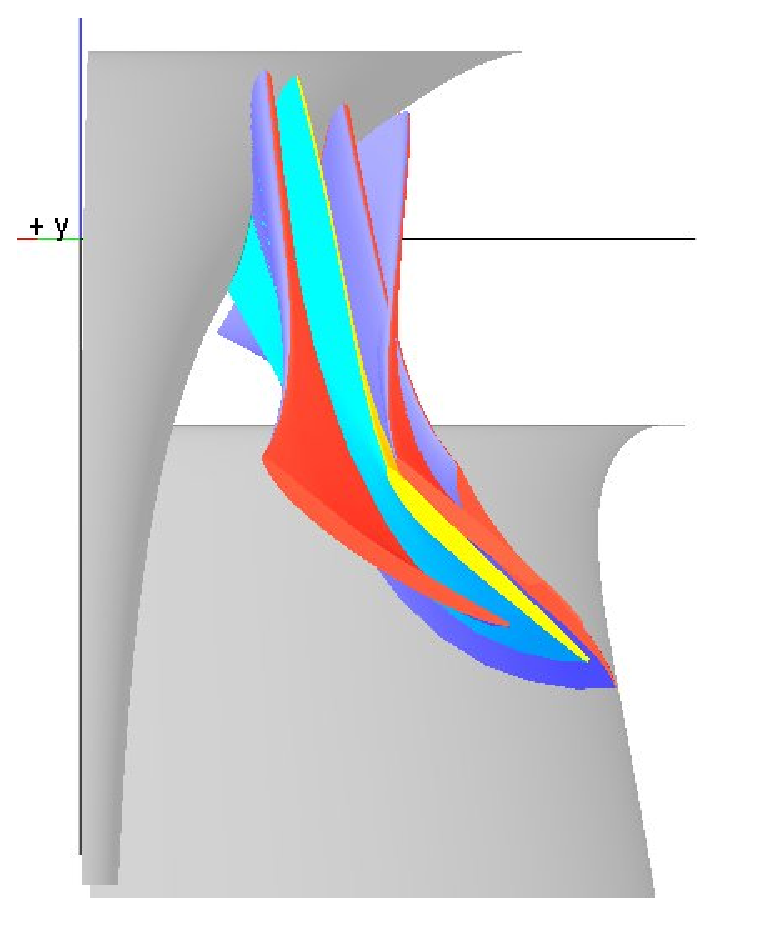
\includegraphics{cbr_r.eps}}
\end{minipage}
\begin{minipage}[b]{0.5\linewidth}
 \centering
 \resizebox*{5cm}{!}{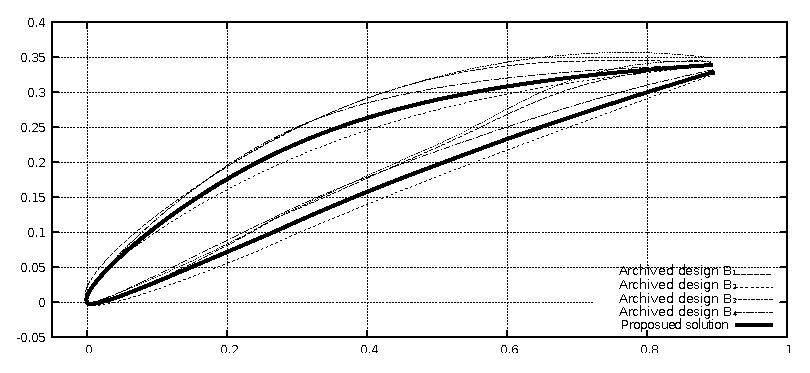
\includegraphics{blade.eps}}
\end{minipage}
\caption{Left: a new Francis blade (light blue and yellow) is designed on the basis of 3 older ones (dark blue and red). Right: a new air-foil (continues line) is designed on the basis of 4 older ones (dotted lines).} 
\label{CBRtemp}
\end{figure}

%\figuremacroW{cbr_r}{Francis CBR}{Here a new Francis blade (light blue and yellow) is designed on the basis of 3 older ones (dark blue and red).}{0.7}

Two applications of KBD, for the design of Francis hydro-turbine and a compressor cascade, are presented in fig.\ref{CBRtemp}. The Francis blade (left) is generated from the KBD method using three design bases (dark blue designs). Using the KBD method a significant  reduction in the design parameters was achieved, form $336$ to 19  ($3$ bases $\times 6$ groups $+1$ extrapolation parameter). The compressor cascade (right) is design using four bases (dotted lines) and the number of design parameters was decreased from 27 to 13 ($4$ bases $\times 3$ groups $+1$ extrapolation parameter).

%As an example of the aforementioned technique firstly the generation of a Francis blade as based on three similar (with respect of Q11 and N11) base blades is shown in fig.\ref{CBRtemp}(left). The new design is the light blue and yellow one and is parameterized with 19 parameters ($3$ bases $\times 6$ groups $+1$ extrapolation parameter). The base designs are parameterized with 336 design variables each using a mean surface plus thickens parameterization (futher ditails about the parameterization are given in Chapter \ref{ParamEval}). Also the generation of a two-dimensional  
\section{Design of a compressor cascade using KBD}
\label{Drela1}
The design of a two dimensional compressor cascade operating at $M_1=0.54$, $a_1=44^o$ and $Re=4\times10^5$ with minimum total pressure losses ($\omega$) is sought. The blade is designed subject to a number of aerodynamic and geometrical constraints, the blade must achieve flow turn greater than $30^o$ and respect the minimum thickness ($0.10/c$, $0.08/c$ \& $0.01/c$) at three chord-wise positions ($0.3$, $0.6$ \& $0.9$) of the airfoil.     

The airfoil shape is parameterized based on a mean-camber line and thickness distributions (suction and pressure side) scheme. Both the mean-camber line and the thickness distributions are parameterized using NURBES curves.  Mean-camber line is parameterized with three variables namely the leading edge (LE) angle, the trailing edge (TE) angle and the weight associated with the middle control point. The suction side thickness distribution is controlled via $9$ design variables, namely the $x$ position, $y$ position and weight of the three, from a total of five, internal nurbs control points, first and last control points are fixed at the LE and TE positions. Pressure side thickness distribution is controlled via 15 design variables namely the $x$ position, $y$ position and weight of the five, from a total of eight, internal control points, first and last control points are fixed at the LE and TE positions and the second point is controlled for the desire of 1st order continuity at LE.  The total number of design variables that describe each candidate solution is $27$ fig.\ref{CBRparam}. 

\begin{figure}[h!]
\begin{minipage}[b]{1\linewidth}
 \centering
 \resizebox*{11cm}{!}{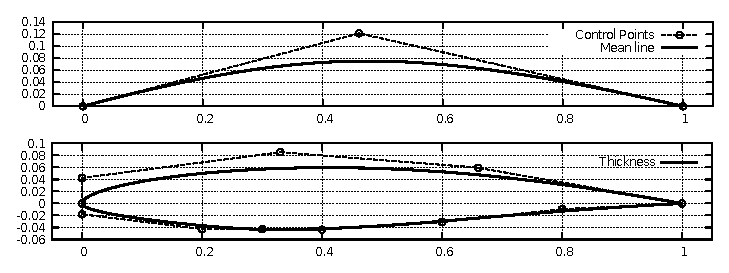
\includegraphics{airf.eps}}
\end{minipage}
\caption{Top: the parametrization of the mean-camber line with $3$ control points. Down: the parametrization of the thickness distributions, $5$ control points for suction side and $8$ control points for pressure side. Total number of design variables is $27$.} 
\label{CBRparam}
\end{figure}

The merits of the KBD method will be examined through the comparison of a traditional MAEA against a KBD-MAEA. The populations for both MAEAs are $\mu=20$, $\lambda=60$ and $\lambda_e=6$. Both cases use local RBFn trained on $10-20$ training patterns. For KBD-MAEA the IPE phase begins after $100$ individuals are stored in the database. On the other hand for the simple MAEA run, $400$ individuals must be stored in the database in order for the IPE phase to begin. The evaluation software is an integral boundary layer method \cite{Drel1987}. The maximum number of calls to the evaluation software was set equal to $1500$.              


Four older "good" designs are chosen as bases. The bases have been designed for operation at different but neighbouring conditions i.e. \textit{base-a} was designed for $M_1=0.55$ and $a_1=45^o$, \textit{base-b} for $M_1=0.50$ and $a_1=40^o$, \textit{base-c} $M_1=0.52$ and $a_1=42.5^o$ and \textit{base-d} for $M_1=0.58$ and $a_1=48^o$. Operating at their design conditions the base geometries perform as follows: \textit{base-a} $\Delta a=37.1^o$ and $\omega=0.01976$, \textit{base-b} $\Delta a=24.4^o$ and $\omega=0.01845$, \textit{base-c} $\Delta a=36.3^o$ and $\omega=0.02027$ and \textit{base-d} $\Delta a=36.6^o$ and $\omega=0.01877$. Reused in the problem specific conditions the aforementioned designs yield $\Delta a=36.3^o$ and $\omega=0.0207$, $\Delta a=27.8^o$ and $\omega=0.0278$, $\Delta a=37.5^o$ and $\omega=0.0201$ and $\Delta a=33.1^o$ and $\omega=0.0237$ respectively. A closer look at both $\omega$ and $\Delta a$ values reveals the necessity for a revise step since all four bases suffer from relatively high losses and some of them fail to respect the $\Delta a$ constraint when used in the new conditions. For the sake of fairness, these four designs were injected in the first generation of the simple MAEA as well.  


\begin{figure}[h!]
\begin{minipage}[b]{1\linewidth}
 \centering
 \resizebox*{11cm}{!}{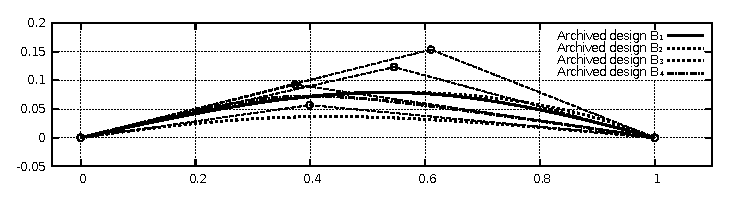
\includegraphics{mean_s.eps}}
\end{minipage}
\caption{Mean-camber line of the four design bases. The big variance between them, forces big design variable range for the optimization procedure that has to, at least, be able to reproduce them and even bigger if extrapolation possibility is sought. This can significantly deteriorate EA efficiency and also deems the use of metamodels not profitable. } 
\label{CBRDmm}
\end{figure}

\begin{figure}[h!]
\begin{minipage}[b]{1\linewidth}
 \centering
 \resizebox*{11cm}{!}{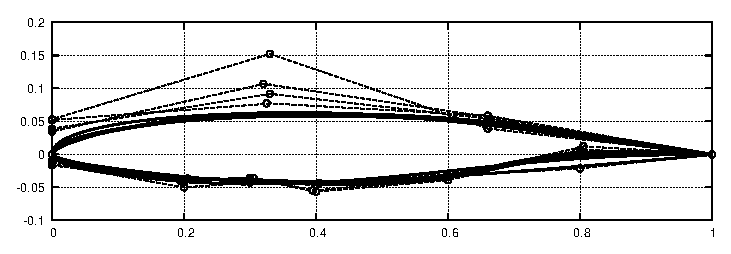
\includegraphics{thickness_s.eps}}
\end{minipage}
\caption{Suction and pressure side thickness distributions and control point polygons for the four geometry bases.} 
\label{CBRDtt}
\end{figure}

Four different optimization procedure were performed in order to asses both the effect of KBD in EA itself and also its effect at the use of metamodels in case of MAEA. The convergence plots are summarized in fig \ref{CBRDrela}. The use of metamodels in the non-KBD runs are not profitable, as expected. This is a result of the very big design space that comes out of the necessity to, at least, have the ability to reproduce the four base geometries (figs \ref{CBRDmm} \& \ref{CBRDtt} ). Using a smaller design space would help both the EA efficiency and the additional gain from the use of metamodels (MAEA) but could result in suboptimal solutions since the optimal geometry could lay outside of the smaller design space. Comparing EA with KBD-EA the merits of the proposed method are obvious (fig. \ref{CBRDrela}), since better and faster convergence is achieved. Furthermore comparing KBD-MAEA with  KBD-EA,  better facilitation of metamodels is observed since the additional gain from their use is noticeable. 

\begin{figure}[h!]
\begin{minipage}[b]{1\linewidth}
 \centering
 \resizebox*{11cm}{!}{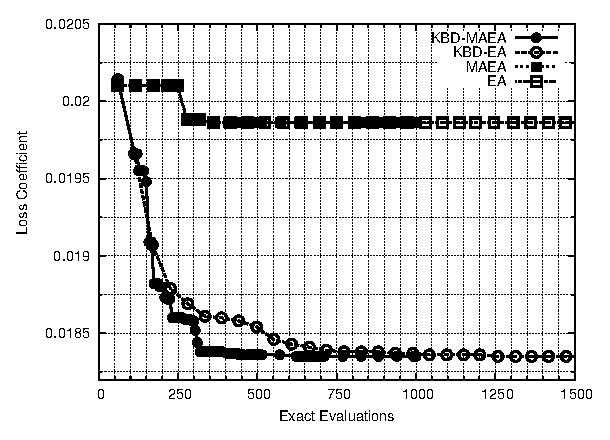
\includegraphics{Comp.eps}}
\end{minipage}
\caption{Convergence comparison of four optimization run, EA vs KBD-EA vs MAEA vs KBD-MAEA. EA and MAEA have similar convergence plots, the use of metamodels does not yield any additional gain due to the big size of the design space. KBD-EA is significantly faster than EA \& MAEA thus proving the merits of the proposed method. Furthermore KBD-MAEA yields additional gain proving the positive effect that the proposed method has also on the use of metamodels.} 
\label{CBRDrela}
\end{figure}

The optimal blade resulting form KBD-MAEA is presented in fig. \ref{CBRDrelaRes}. The design delivers $\omega=0.01834$ and $\Delta a = 30.2^o$ at the desirable conditions. The design is better than all basis design (operating at the desirable conditions) and respects all the constraints. The delivered form KBD-MAEA design is also of significantly better quality than the designs delivered by all the non-KBD optimization procedures. 

\begin{figure}[h!]
\begin{minipage}[b]{1\linewidth}
 \centering
 \resizebox*{14cm}{!}{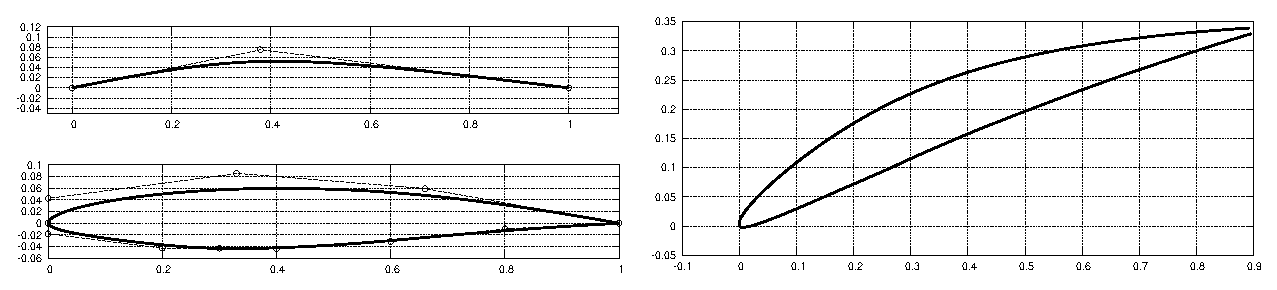
\includegraphics{ResD.eps}}
\end{minipage}
\caption{The optimal blade resulting form KBD-MAEA. Left: mean camper line and thickness distribution together with their control polygons. Right: The final blade after superimposing thickness distribution on the mean camper line and turned accordingly with the stagger angle.} 
\label{CBRDrelaRes}
\end{figure}


% ---------------------------------------------------------------------------
% ----------------------- end of thesis sub-document ------------------------
% ---------------------------------------------------------------------------
